\RequirePackage{fix-cm}
\documentclass[smallextended]{svjour3}       % onecolumn (second format)
\smartqed  % flush right qed marks, e.g. at end of proof
\usepackage{graphicx,multicol,lipsum,caption,authblk} 
\usepackage{amsmath,verbatim,tikz}
\usepackage{geometry,pgf,pgfplots,}
\usepackage{mathptmx}
\usepackage{booktabs, makecell, multirow, threeparttable}
\usepackage{tablefootnote}
\usetikzlibrary{shapes.geometric, arrows,positioning,matrix,calc}
\usetikzlibrary{intersections}
\bibliographystyle{unsrtnat}
% in order to solve arranging citations by order of appearance
\usepackage[numbers]{natbib}
\usepackage{notoccite}

\captionsetup{figurename=Figure,tablename=Table}
\setlength\parindent{8pt}

\begin{document}

\title{Automation Design of Artificial Neural Network by Genetic Algorithm}
%\titlerunning{Stacking Sequence Optimization}        % if too long for running head
\author{Zhang Huiyao$^1$  \and
	Atsushi Yokoyama $^{1,*}$
}
\authorrunning{Zhang Huiyao} % if too long for running head
\institute{Zhang Huiyao \at
              Room 203,Bulding 3,Kyoto Institue of Technology\\
			  Matsugasaki,Sakyo-ku,Kyoto,606-8585,JAPAN\\
              \email{zhanghy1012@gmail.com}           %  \\
           \and
           S. Author \at
              second address
}
\date{Received: date / Accepted: date}
\maketitle

\begin{abstract}
	Based on Ockham's razor, the more complexity your model is, the greater the
	possibility for errors are. to keep the model as simple as possible. In this
	paper, genetic algorith method is used to search the simplest neural network
	strucutre for a specific problem. The experiment result has shown that a
	simpler neural network can always be found, and the neural network can also
	be used to compress original data.
\keywords{Genetic Algorithm \and Neural Network Design \and Automation }
\end{abstract}

\begin{multicols}{2}
\section{Introduction}
The structure of a neuron, as shown in Figure.\ref{fig:neuron}, is pretty simple
and intuitive, it is consists of dendrites, synapse, cell body, and axon. The
number of neurons in human body is about $10^{11}$,  based on the repeat of this
simple neuron pattern, a human being can do reasoning, learning, memorizing, and
visualizing.  To mimick the behavior of neuron, many neural network have been
designed.  Hammming network is used to solve binary pattern recognition problem.
Hopfield\cite{hopfield1982neural} network is used to solve memorizing problem.
Grossberg Network\cite{grossberg1976adaptive} is used to solve vision
recognition problem.  So many amazing neural networks have been developed,
however, there isn't a systematic approach to guide the design of neural
network.  Murata\cite{murata1994network} proposed pruning method to decide
whether or not should include a neuron.  Some researchers\cite{demuth2014neural}
use growing methods to build the neural network.\\ 

In this paper, global search method is used to find the simplest neural network
that can explains the data.


\begin{center}
  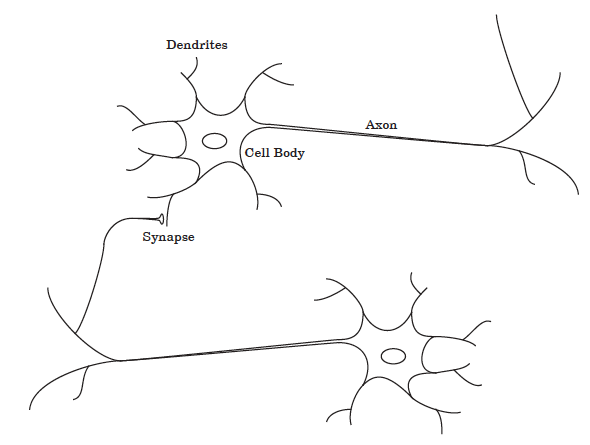
\includegraphics[width=\linewidth]{neural_network_design_images/neuron1.png}
  \captionof{figure}{Schematic Drawing of Biological Neurons}
  \label{fig:neuron}
\end{center}

Genetic algorithms (GAs) are first introduced in 1975 by
Holland\cite{goldberg1987genetic} because of its powerful search ability,
which was widely been used to solve many search, optimiation, and classification
problem. Compared with other random search algorithm, for example, particle
swarm optimization, ant colony optimization, and simulated annealing
algorithm, GAs are not easily trapped in local optima,
and obtain the global optimal. 
\vspace{2pt}
\begin{center}
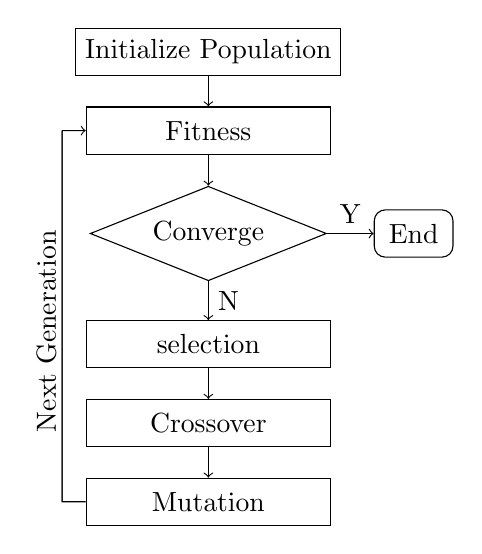
\begin{tikzpicture}
\tikzstyle{startstop} = [rectangle, rounded corners, minimum width=1.0cm,minimum height=0.6cm, 
                        text centered, draw=black]
\tikzstyle{io} = [trapezium, trapezium left angle=70, trapezium right angle=110, minimum width=2cm, 
                 minimum height=0.6cm, text centered, draw=black]
\tikzstyle{process} = [rectangle, minimum width=3.1cm, minimum height=0.6cm, text centered, draw=black]
\tikzstyle{decision} = [diamond,minimum width=3cm, minimum height=1.2cm, draw=black]
\node (population) [process] {Initialize Population};
\node (fitness) [process, below of=population] {Fitness};
\node (decision) [decision] at ($(fitness.south)+(0,-1.0cm)$) {} node at (decision.base) {Converge};
\node (share-fitness) at ($(decision.south)+(0,-0.8cm)$) [process] {selection};
\node (selection) [process,below of=share-fitness] {Crossover};
\node (crossover) [process,below of=selection]  {Mutation};
%\node (mutation) [process,below of=crossover]   {Mutation};
\node (end) [startstop] at ($(decision.east)+(1.1cm,0)$)  {End};

\draw [->] (population) -- (fitness);
\draw [->] (fitness) -- (decision);
\draw [->] (decision) -- (share-fitness) node[auto=left,pos=0.5]{N};
\draw [->] (share-fitness.south) -- (selection.north) ;
\draw [->] (selection.south) -- (crossover.north);
%\draw [->] (crossover.south) -- (mutation.north);
\draw [->] (decision.east) -- (end.west) node[auto=left,pos=0.5]{Y};

% draw intersection
\draw [white] (fitness.west) -- ++(-0.5cm,0) coordinate (A);
\draw [white] (crossover.west) -- ++(-0.3cm,0) coordinate (B)-- ++(0,6cm) coordinate (C) ; 
\draw (crossover.west) -- ++(-0.3cm,0) -- (intersection cs: first line={(fitness.west)--(A)}, 
      second line={(B)--(C)}) coordinate (D);
\draw (B) -- (D) node[auto=left,pos=0.8,rotate=90,xshift=-0.2cm,yshift=0.2cm] {Next Generation} ;
\draw [<-] (fitness.west) -- (D);
\end{tikzpicture}
\captionof{figure}{Genetic Algorithm}
\end{center}

\begin{comment}
\begin{center}
  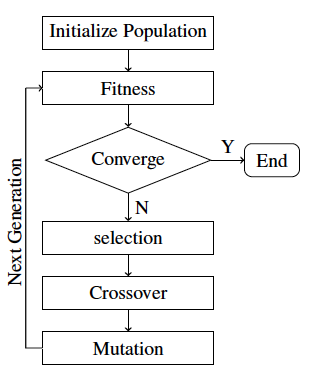
\includegraphics[width=\linewidth]{neural_network_design_images/ga.png}
  \captionof{figure}{Genetic Algorithm}
  \label{fig:genetic_algorithm}
\end{center}
\end{comment}

\section{Problem-oriented Neural Network Model}
For a specific engineering problem, the inputs and outputs of the neural
network are fixed. The design problem unsolved is the number of hidden layers ,
the number of nodes in each hidden layer, and the transfer functions. Accordint to
Ockham's razor, the simple model are more likely to be the right one, so in this
paper, one principal is to keep the neural network as simple as possible. The
more number of hidden layers, the more complexity the model is. Actually, a
two-layer network can approximate any practical function, so there is only one
hidden layer in the neural network model.


According to Karlik's\cite{karlik2011performance} research, the performance of
neural network not only based one the architecture, but also related to the
transfer fucntions. Mostly used transfer functions such as  sigmoid, relu, tanh and
softmax function are discussed in this paper. In order to discuss transfer
function in genetic algorithm,  different bianry codes are used to indicate
transfer function.  '00' stands for sigmoid function, '01' for relu function,
'10' for tanh function, and '11' for softmax function, as shown in Table
\ref{tab:transfer function}


\begin{center}
\captionof{table}{Transfer Function}
\begin{tabular}{ccc}
	\toprule
	Name 				 & Equation                                   & Binary
	code\\
	\midrule
	sigmoid              & $ f(x)=\frac{1}{1+e^{-x}} $  & $00$ \\
	relu                 & $ f(x)=\max \{0, x\} $       & $01$ \\
	tanh                 & $
	f(x)=\frac{\left(e^{x}-e^{-x}\right)}{\left(e^{x}+e^{-x}\right)} $&
	$10$ \\
	softmax                 & $
	f(x_i)=\frac{e^{x_i}}{\sum_{i=1}^{K} e^{x_i}}
							$ & $11$ \\
	\bottomrule
\end{tabular}
\label{tab:transfer function}
\end{center}



Each neuron in hidden layer can be treated as a feature extractor, which is
randomly connected with the inputs.  As the output of the neural network fully 
depend on the features that the neural network learnt, the output layer and
the hidden layer should be full connected.  So the potential neural network
model is as shown in Figure.\ref{plot:neural_network_model} 





As shown in Figure.\ref{plot:neural_network_model} \\
1. Neurons in the output layer are full connected with the neurons in the
hiddern layer. \\
2. Every neuron in the hiddern layer is partially connected with the input, for
example $b_1$ only connects with $a_1, a_2$\\ 
3. The number of neurons $m$ is randomly initialized and m is greater then 1 and
less then n \\
\section{Genetic Algorithm Procedure}
\subsection{Population Initialization}
As showned in figure.\ref{plot:neural_network_model}, neurons in hidden layer are
randomly connected with the inputs. If there is a connection between previous
neuron and current neuron, it is indicated by a constant numberic value 1, otherwise the
number is 0 which means no connection. This process can be divided into two
steps:
\begin{enumerate}
	\item random generate the number of nodes in the hidden layer, denoted by $m$.
	\item generate the chromosome, the length is $ m \times l$, $l$ denotes the
		lenght of each locus.
\end{enumerate}

For example, assuming the random number $m$ is 4 and the corresponding
chromosome is $110100 \text{ }\text{ }011101\text{ }\text{ } 010101 \text{ }\text{ }010110$. The chromosome can be divided into
four parts, each part corresponds to the locus of one node in the hidden layer;
each part can be divided into two subparts, the length of each locus is 6, the
beginning four parts indicate the connection, the last 2 bits stand for 
transfer function. So the architecture of this neural network is as
shown in Figure \ref{plot:neural_network_model_example}(a).  \\

In Figure \ref{plot:neural_network_model_example}(b), there are two nodes in the
hiddern layer, so the beginning four parts of locus of neuron $h_1$ and $h_2$
are $1 1 0 1 $, $0 0 1 1$. 

\begin{center}
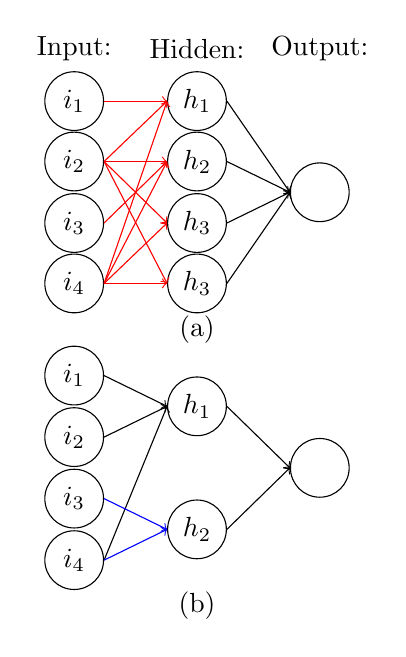
\begin{tikzpicture}
[ plain/.style={ draw=none, fill=none, }, remember picture, net/.style={ matrix of nodes, nodes={ draw, circle,
    inner sep=7.5pt
    },
  nodes in empty cells,
  column sep=0.8cm,
  %column sep=-10.5pt,
  %row sep=0.8cm
  row sep=-10.5pt
  }
]
%\draw[help lines] (-3cm,-6cm) grid (6cm,3cm);
\matrix[net] (mat)
{
              &           &  |[plain]|                      \\
    |[plain]| & |[plain]| &  |[plain]|                      \\ 
			  & 		  &  |[plain]|                      \\ 
    |[plain]| & |[plain]| &                                 \\
              &           &  |[plain]|                      \\
    |[plain]| & |[plain]| &  |[plain]|                      \\
              &           &  |[plain]|                      \\
  };

 \foreach \a in {1,3,7}{
        \draw[->,red] (mat-\a-1.east) -- (mat-1-2.west);
  }

 \foreach \a in {3,5,7}{
        \draw[->,red] (mat-\a-1.east) -- (mat-3-2.west);
  }

 \foreach \a in {3,7}{
        \draw[->,red] (mat-\a-1.east) -- (mat-5-2.west);
  }

 \foreach \a in {3,7}{
        \draw[->,red] (mat-\a-1.east) -- (mat-7-2.west);
  }

 \foreach \a in {1,3,5,7}{
        \draw[->] (mat-\a-2.east) -- (mat-4-3.west);
  }
  \node at ($(mat-7-2.south)+(0,-0.2cm)$) {(a)};
  \node at ($(mat-1-1.north)+(0, 8pt)$) {Input: };
  \node at ($(mat-1-2.north)+(0, 8pt)$) {Hidden:};
  \node at ($(mat-1-3.north)+(0, 8pt)$) {Output:};
  \node at (mat-1-1.base) {$i_1$};
  \node at (mat-3-1.base) {$i_2$};
  \node at (mat-5-1.base) {$i_3$};
  \node at (mat-7-1.base) {$i_4$};
  \node at (mat-1-2.base) {$h_1$};
  \node at (mat-3-2.base) {$h_2$};
  \node at (mat-5-2.base) {$h_3$};
  \node at (mat-7-2.base) {$h_3$};

  \begin{scope}[shift={(0,-3.5cm)}]
	\matrix[net] (mat)
	{
				  & |[plain]| &  |[plain]|                      \\
		|[plain]| &           &  |[plain]|                      \\ 
				  & |[plain]| &  |[plain]|                       \\ 
		|[plain]| & |[plain]| &                                 \\
				  & |[plain]| &  |[plain]|                      \\
		|[plain]| &           &  |[plain]|                      \\
				  & |[plain]| &  |[plain]|                      \\
	  };

 \foreach \a in {1,3,7}{
        \draw[->] (mat-\a-1.east) -- (mat-2-2.west);
  }
 \foreach \a in {5,7}{
        \draw[->,blue] (mat-\a-1.east) -- (mat-6-2.west);
  }

 \foreach \a in {2,6}{
        \draw[->] (mat-\a-2.east) -- (mat-4-3.west);
  }
  \node at (mat-1-1.base) {$i_1$};
  \node at (mat-3-1.base) {$i_2$};
  \node at (mat-5-1.base) {$i_3$};
  \node at (mat-7-1.base) {$i_4$};
  \node at (mat-2-2.base) {$h_1$};
  \node at (mat-6-2.base) {$h_2$};

  \node at ($(mat-7-2.south)+(0,-0.2cm)$) {(b)};
  \end{scope}
\end{tikzpicture}
\captionof{figure}{Neural Network Example}
\label{plot:neural_network_model_example}
\end{center}

\subsection{Selection}
Ranking selection is taken to choose the parents of next generation from high to
low according to their fitness. The individual with best fitness are choosen as
parents, repeat the process until you get the desired amount of population. \\

  The input data is splitted into two parts, training data and evaluation data,
traing data is used to adjust the parameters in the neural network, and
evaluation data is used to measure the performance of the neural network. The
performance of the neural network on evaluation data is treated as the fitness
of the neural network, as shown in Figure \ref{plot:ga_and_nn}.

\begin{center}
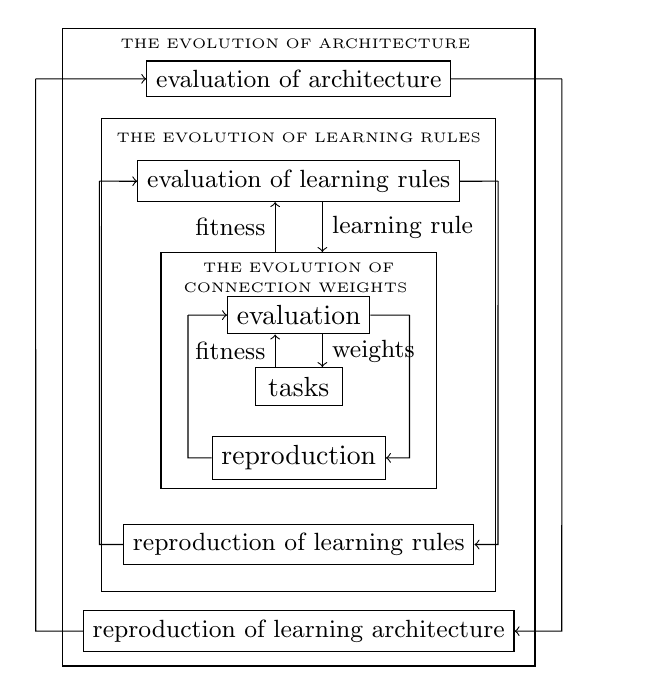
\begin{tikzpicture}
    %\draw[help lines] (-3cm,-6cm) grid (6cm, 6cm);
    \tikzstyle{block} = [rectangle, text centered, draw=black,
    minimum width=1.1cm, minimum height=0.4cm]
%    \draw[white] (4,4.5) rectangle (5,5.6);
    
    % first level
    \node (evaluation-parent) [block, minimum width=2.4cm, minimum
        height=1.8cm,draw=white] {};
    \node (evaluation) [block] at ($(evaluation-parent.north)$) {evaluation};
    \node (reproduction) [block] at ($(evaluation-parent.south)$) {reproduction};
    \node (tasks) [block, minimum width=1.1cm, minimum height=0.4cm] {tasks};


    \draw[->] ($(evaluation.south)+(0.3cm,0cm)$) --
        ($(tasks.north)+(0.3cm,0cm)$) node[auto=left, pos=0.5] {\small weights}; 
    \draw[<-] ($(evaluation.south)+(-0.3cm,0cm)$) --
        ($(tasks.north)+(-0.3cm,0cm)$) node[auto=right, pos=0.5] {\small fitness}; 

    % get intersection
    \draw[white] (evaluation.west) coordinate (A) -- ++(-1.5cm,0) coordinate (B);
    \draw[white] (reproduction.west) -- ++(-0.3cm,0) coordinate (C) -- ++(0,4cm) coordinate
        (D);
    \draw[black] (reproduction.west) -- ++(-0.3cm,0) -- (intersection cs:
        first line={(A)--(B)}, second line={(C)--(D)}) coordinate (E);
    \draw[->] (E) -- (evaluation.west);

    \draw[white] (evaluation.east) coordinate (E) -- ++(2cm,0) coordinate (F);
    \draw[white] (reproduction.east) -- ++(0.3cm,0) coordinate (G) -- ++(0,4cm) coordinate
        (H);
    \draw[<-] (reproduction.east) -- ++(0.3cm,0) -- (intersection cs:
        first line={(E)--(F)}, second line={(G)--(H)}) coordinate (I);
    \draw (I) -- (evaluation.east);

    % second level
    \node (level2) [block,draw=black, minimum width=3.5cm, minimum height=3.0cm] at
        (0cm,0.2cm) {};
    \node [align=left] at ($(level2.north)+(0,-0.2cm)$) {\tiny THE EVOLUTION
        OF};
    \node [align=left] at ($(level2.north)+(0,-0.45cm)$) {\tiny CONNECTION
            WEIGHTS 
        };
    % third level
    \node (level3-assister) [block, draw=white, minimum width=5cm, minimum
		height=4.6cm] at
        (0, 0.3cm)  {};
    \node (evaluation) [block] at ($(level3-assister.north)$) {\small evaluation of
        learning rules};
    \node (reproduction) [block] at ($(level3-assister.south)$) {\small reproduction of
        learning rules};

    \draw[->] ($(evaluation.south)+(0.3cm,0cm)$) --
        ($(level2.north)+(0.3cm,0cm)$) node[auto=left, pos=0.5] {\small learning
        rule}; 
    \draw[<-] ($(evaluation.south)+(-0.3cm,0cm)$) --
        ($(level2.north)+(-0.3cm,0cm)$) node[auto=right, pos=0.5] {\small fitness}; 

    \draw[white] (evaluation.west) coordinate (A) -- ++(-1.3cm,0) coordinate (B);
    \draw[white] (reproduction.west) -- ++(-0.3cm,0) coordinate (C) -- ++(0,4cm) coordinate
        (D);
    \draw[black] (reproduction.west) -- ++(-0.3cm,0) -- (intersection cs:
        first line={(A)--(B)}, second line={(C)--(D)}) coordinate (E);
    \draw[->] (E) -- (evaluation.west);

    \draw[white] (evaluation.east) coordinate (E) -- ++(2cm,0) coordinate (F);
    \draw[white] (reproduction.east) -- ++(0.3cm,0) coordinate (G) -- ++(0,4cm) coordinate
        (H);
    \draw[<-] (reproduction.east) -- ++(0.3cm,0) -- (intersection cs:
        first line={(E)--(F)}, second line={(G)--(H)}) coordinate (I);
    \draw (I) -- (evaluation.east);
   % fourth level
    \node (level4) [block, draw=black, minimum width=5.0cm, minimum
        height=6.0cm] at
        (0, 0.4cm)  {};
    \node [align=left] at ($(level4.north)+(0,-0.25cm)$) {\tiny THE EVOLUTION
        OF LEARNING RULES};
    % level five
    \node (level5-assister) [block, draw=white, minimum width=6.4cm, minimum
        height=7.0cm] at
        (0, 0.4cm)  {};
    \node (evaluation) [block] at ($(level5-assister.north)$) {\small evaluation of
        architecture};
    \node (reproduction) [block] at ($(level5-assister.south)$) {\small reproduction of
        learning architecture};

    \draw[white] (evaluation.west) coordinate (A) -- ++(-1.5cm,0) coordinate (B);
    \draw[white] (reproduction.west) -- ++(-0.6cm,0) coordinate (C) -- ++(0,4cm) coordinate
        (D);
    \draw[black] (reproduction.west) -- ++(-0.6cm,0) -- (intersection cs:
        first line={(A)--(B)}, second line={(C)--(D)}) coordinate (E);
    \draw[->] (E) -- (evaluation.west);

    \draw[white] (evaluation.east) coordinate (E) -- ++(2cm,0) coordinate (F);
    \draw[white] (reproduction.east) -- ++(0.6cm,0) coordinate (G) -- ++(0,4cm) coordinate
        (H);
    \draw[<-] (reproduction.east) -- ++(0.6cm,0) -- (intersection cs:
        first line={(E)--(F)}, second line={(G)--(H)}) coordinate (I);
    \draw (I) -- (evaluation.east);
    % level 6
    \node (level6) [block, minimum width=6.0cm, minimum
        height=8.1cm] at
        (0, 0.5cm)  {};
    \node [align=left] at ($(level6.north)+(0,-0.2cm)$) {\tiny THE EVOLUTION OF
            ARCHITECTURE
        };
\end{tikzpicture}
\captionof{figure}{Genetic Algorithm and Neural Network}
\label{plot:ga_and_nn}
\end{center}

\subsection{Crossover}
  The crossover is a little bit different from traditional genetic algorithm,
because the length of chromosomes which are chosen as parents maybe  not
equal.  So the following rule is used for crossover operation,  take 
half number of loci in each chromosome, and combine these loci into a new
chromosome \\
  For example, networks as shown in Figure
\ref{plot:neural_network_model_example}(a) and
Figure \ref{plot:neural_network_model_example}(b) , the number of loci in the
hidden layer in each network are 4 and 2, so the number of loci of their
offspring is 3. At the same time, the offspring also inherit connection
relationship and transfer function from their parents. As shown in Figure
\ref{plot:offspring}, the red color connection inheirts from network in Figure
\ref{plot:neural_network_model_example}(a) and the blue connection inherits from
network in Figure \ref{plot:neural_network_model_example}(b)\\ 

\begin{center}
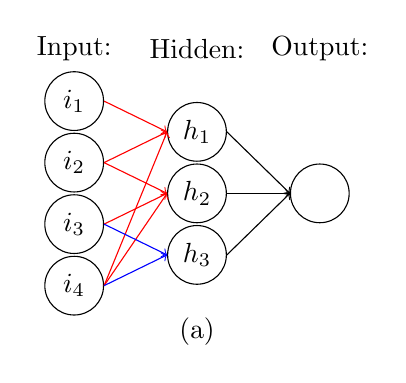
\begin{tikzpicture}
[ plain/.style={ draw=none, fill=none, }, remember picture, net/.style={ matrix of nodes, nodes={ draw, circle,
    inner sep=7.5pt
    },
  nodes in empty cells,
  column sep=0.8cm,
  %column sep=-10.5pt,
  %row sep=0.8cm
  row sep=-10.5pt
  }
]
%\draw[help lines] (-3cm,-6cm) grid (6cm,3cm);
\matrix[net] (mat)
{
              & |[plain]| &  |[plain]|                      \\
    |[plain]| &           &  |[plain]|                      \\ 
			  & |[plain]| &  |[plain]|                      \\ 
    |[plain]| &           &                                 \\
              & |[plain]| &  |[plain]|                      \\
    |[plain]| &           &  |[plain]|                      \\
              & |[plain]| &  |[plain]|                      \\
  };

 \foreach \a in {1,3,7}{
        \draw[->,red] (mat-\a-1.east) -- (mat-2-2.west);
  }

 \foreach \a in {3,5,7}{
        \draw[->,red] (mat-\a-1.east) -- (mat-4-2.west);
  }

 \foreach \a in {5,7}{
        \draw[->,blue] (mat-\a-1.east) -- (mat-6-2.west);
  }


 \foreach \a in {2,4,6}{
        \draw[->] (mat-\a-2.east) -- (mat-4-3.west);
  }
  \node at ($(mat-7-2.south)+(0,-0.2cm)$) {(a)};
  \node at ($(mat-1-1.north)+(0, 8pt)$) {Input: };
  \node at ($(mat-1-2.north)+(0, 8pt)$) {Hidden:};
  \node at ($(mat-1-3.north)+(0, 8pt)$) {Output:};
  \node at (mat-1-1.base) {$i_1$};
  \node at (mat-3-1.base) {$i_2$};
  \node at (mat-5-1.base) {$i_3$};
  \node at (mat-7-1.base) {$i_4$};
  \node at (mat-2-2.base) {$h_1$};
  \node at (mat-4-2.base) {$h_2$};
  \node at (mat-6-2.base) {$h_3$};

\end{tikzpicture}
\captionof{figure}{Offspring}
\label{plot:offspring}
\end{center}



\section{Experiment and Results}
Heart disease date set is used to check the performance of this neural network
design method. This dataset was obtained from UCI machine learning benchmark
repository
\subsection{Data Set}
  The data set is used to explore the relationship between the symptoms of a
patient and the presence of heart disease. There are 75 attributes for each
patient, 13 attributes are used as the inputs of the neural network, and 1 is as
the output of neural network. The number of the database is 303, 240 of them are
used as the train data, the remaining is used as the evaluation data.

\subsection{Experiment}
Because data set has 13 attributes as inputs, so each locus has 15 bits. The
beginning 13bits represent the connection, the last two bits stand for transfer
function, relevant parameters as shown in Table \ref{tab:experiment}  

\begin{center}
\begin{tabular}{cc}
	\toprule
	Parameter &  Value \\
	\midrule
	population  & 10         \\ 
	locus length& 15 	      \\
	encoding method & binary          \\
	crossover strategy & one-point \\
	mutation strategy& random\\
	\bottomrule
\end{tabular}
\captionof{table}{Genetic Parameters}
\label{tab:experiment}
\end{center}


\subsection{Results}
The top four neural networks ranked by accurate, as shown
in Table \ref{tab:result}
\captionof{table}{Result}
\begin{tabular}{cccc}
	\toprule
	\makecell{Network \\ Name}   & \makecell{Number of \\Hidden Node} &
	\makecell{Transfer\\ Function} & Accuracy \\
	\midrule
	$n_1$  &4      & R\tablefootnote{Footnote 1}F\tablefootnote{Footnote 2}FF	       &  0.817   \\
	$n_2$  &4      & T\tablefootnote{Footnote 3}S\tablefootnote{footnote 4}RF	         &  0.817   \\
	$n_3$  &3      & TSR &  0.800   \\
	$n_4$  &6      & FFTRFF	         &  0.800   \\
	\bottomrule
\end{tabular}
\begin{tablenotes}\footnotesize
\item  $^1$ R denotes relu function, $^2$ F denotes softmax function, $^3$ T 
	denotes tanh 
function, $^4$ S denotes sigmoid function.  
\end{tablenotes}
\label{tab:result}



\begin{center}
\captionof{table}{Chromosome $n_1$}
\begin{tabular}{cc}
	\toprule
	locus& Binary Presentation \\
	\midrule
	$l_1$  & 0 0 1 0 1 0 1 1 \textcolor{yellow}{0 0} 0 0 1 1 0                 \\
	$l_2$  & 0 1 0 1 0 1 1 0 \textcolor{yellow}{0 0} 0 1 1 0 0     			   \\
	$l_3$  & 1 0 1 0 1 1 0 0 \textcolor{yellow}{0 0} 1 1 0 0 1                 \\
	\bottomrule
\end{tabular}
\label{tab:chromosome1}
\end{center}


As shown in Table \ref{tab:chromosome1}, the two columns which are highlighted
are all zero, it means no neuron in the hidden layer is connected with these two
inputs.


\begin{comment}
\begin{center}
\captionof{table}{Chromosome $n_2$}
\begin{tabular}{cc}
	\toprule
	locus  & Binary Presentation\\
	\midrule
	$l_1$  &   0 1 0 1 1 1 0 1 1 1 0 1 1 0 1               \\
	$l_2$  &   1 0 1 1 1 0 1 1 1 0 1 1 1 1 1   			   \\
	$l_3$  &   0 1 1 1 0 1 1 1 0 1 1 1 1 1 1               \\
	$l_4$  &   1 1 1 0 1 1 1 0 1 1 1 1 1 1 1               \\
	\bottomrule
\end{tabular}
\label{tab:GA}
\end{center}
\end{comment}


\section{Conclusion}
Through automation design of neural network, a simpler architecture can always
be found which can explain the data well. According to the final neural network
be obtained, it can be used to reduce the dimensionality of the input, namely,
data compression. 


%\section{Acknowledgements}
%This is work was supported by China Schloarship Council(CSC).
%\bibliographystyle{plain}
\bibliography{neural-network-design-database}
\end{multicols}

\end{document}
